\chapter{Conductance in the Kondo Regime}\label{cha:kondo_conductance}


\epigraph{Ní dhéanfaidh smaoineamh an treabhadh duit.}{Irish proverb}


\section{Introduction}
\noindent This chapter serves as an introduction to the Kondo effect. The history of the Kondo effect began with a measurement that noticed a strange behaviour (resistivity minimum with decreasing temperature) in impure gold wires. It took thirty years before Jun Kondo explained this effect, hence the name `Kondo effect'. After another thirty years, advancements in technology found the quantum dot an exciting platform to explore the Kondo effect due to its high degree of in-situ tunability. 


% \afterpage{\clearpage}
\section{Kondo Effect in Bulk Materials}


In the 1930s, it was found that the resistivity would surprisingly increase in impure gold wires at low temperatures~\cite{de_haas}. This was unexpected as due to electron-phonon scattering, the resistivity should decrease with $\mathrm{T^5}$ before saturating at some non-zero resistivity. Data from the original experiment is plotted in Fig.~\ref{fig:ch2/kondo_bulkmetal} with expected electron-phonon dependence. Over the coming years, it was found that metals with magnetic impurities had a similar behaviour~\cite{still_irresistible}.


\begin{figure}[!hbt]
 \begin{center}
%% includegraphics: comment the following if not using the graphicx package
  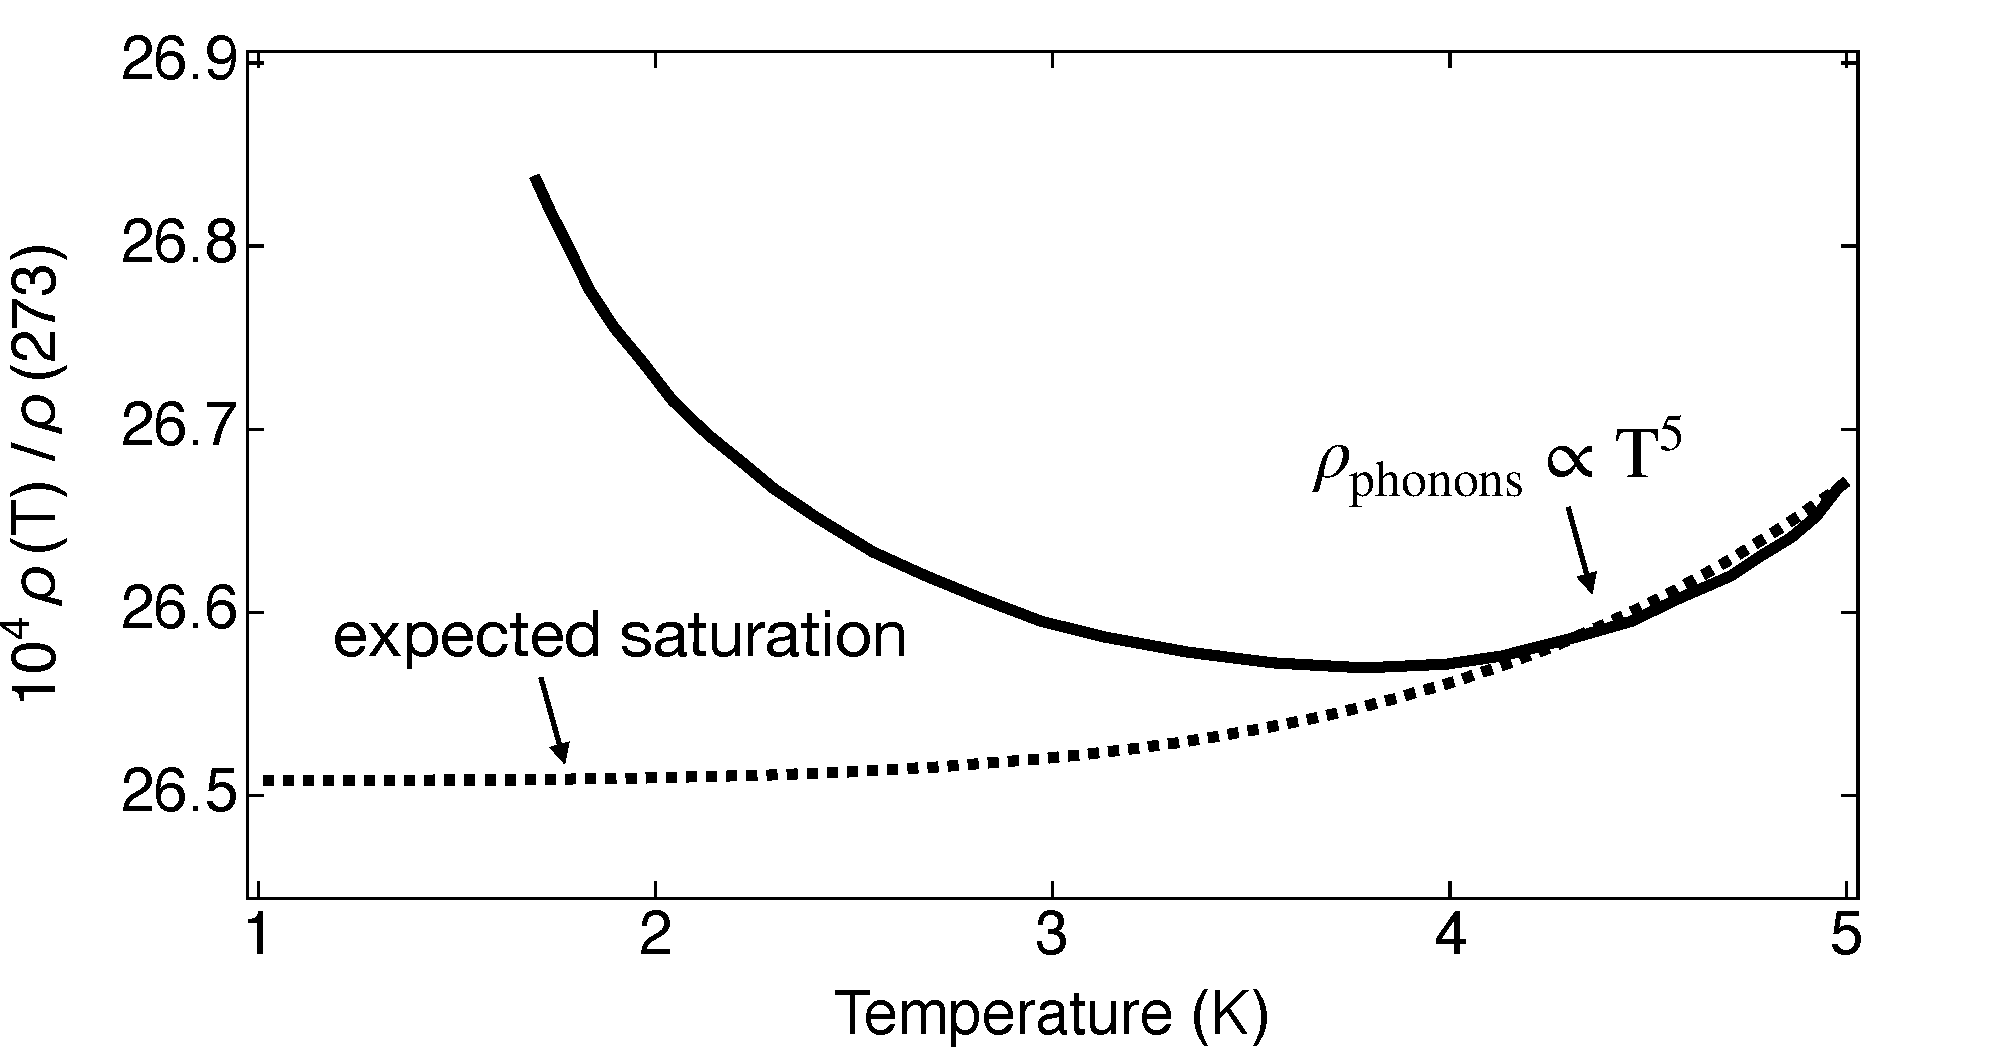
\includegraphics[width=0.9\textwidth]{figures/ch2/figure9.pdf}
  \caption[Kondo Effect in Bulk Materials]{\label{fig:ch2/kondo_bulkmetal} 
  % For some options that work with pdf\LaTeX, please see this discussion:
  %  \url{http://tex.stackexchange.com/questions/11839}. 
  Temperature dependence of the resistivity, $\mathrm{\rho}$. Expectedly, the resistivity initially decreases as $T^5$ due to electron-phonon scattering. However, due to the Kondo effect, the resistivity reaches a minimum before increasing logarithmically with decreasing temperature. The data used for this figure was obtained from~\cite{de_haas}.
   }
 \end{center}
\end{figure}




It took until 1964 for a theoretical explanation of the resistivity minimum~\cite{jun_kondo}. Jun Kondo used the s-d model, which couples a metal (non-magnetic, s-band) to a magnetic impurity (unfilled d-level). By looking at higher-order contributions to the resistivity, a logarithmic term appears, resulting in a large correction at low $\mathrm{T}$. This contribution comes from a process where spin exchange interactions occur. This work showed that a magnetic impurity at low temperatures can give rise to an alternative scattering process, involving a temporary exchange of spin states between the magnetic impurity and surrounding conduction electrons. 

\begin{figure}[!hbt]
 \begin{center}
%% includegraphics: comment the following if not using the graphicx package
  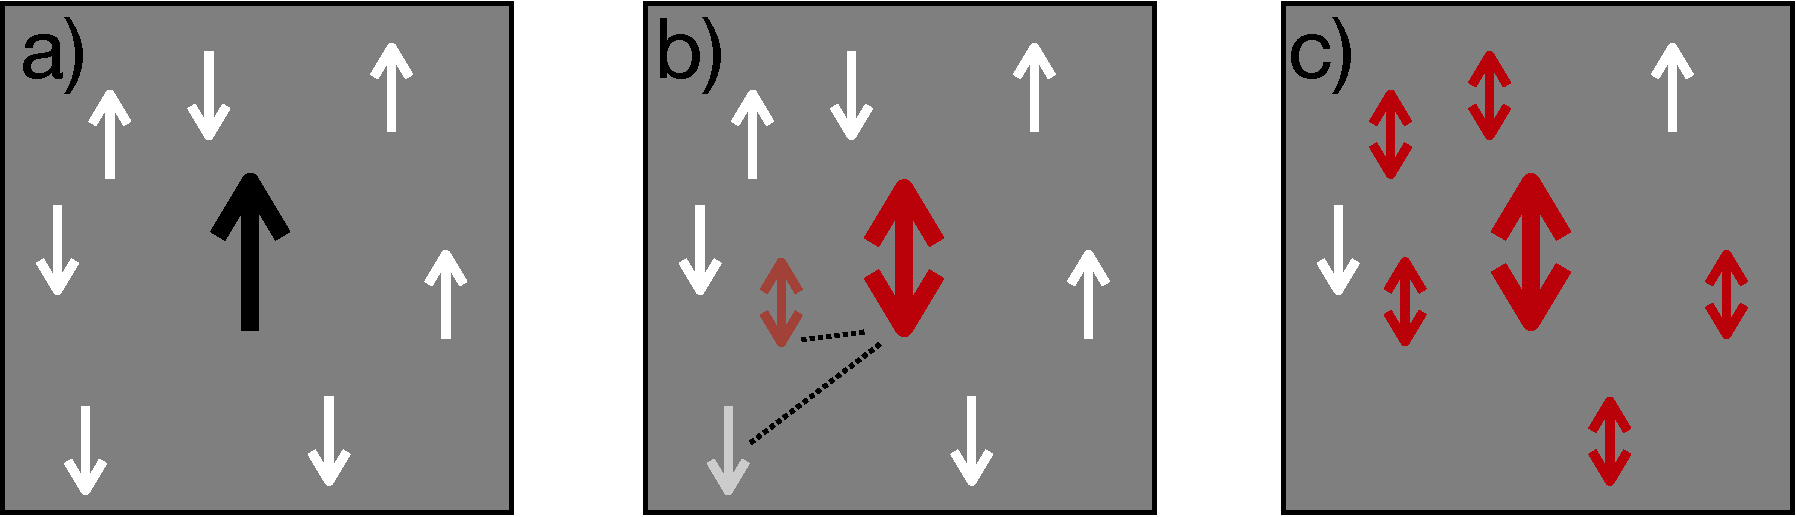
\includegraphics[width=0.9\textwidth]{figures/ch2/figure10.pdf}
  \caption[Kondo Effect Illustration : Bulk Material]{\label{fig:ch2/kondo_bulkdiagram} 
  % For some options that work with pdf\LaTeX, please see this discussion:
  %  \url{http://tex.stackexchange.com/questions/11839}. 
  (\textbf{a}) A single magnetic impurity (black arrow) is surrounded by conduction electrons (white arrow). (\textbf{b}) Conduction electrons scatter off the magnetic impurity, resulting in a possible spin flip of both particles. This leaves the particles entangled. (\textbf{c}) Continued scattering events build a macroscopic coherent state known as a `Kondo singlet'.
   }
 \end{center}
\end{figure}


Fig.~\ref{fig:ch2/kondo_bulkdiagram} illustrates how an exchange of spin states can build a coherent state between the magnetic impurity and the free conduction electrons. It begins with Fig.~\ref{fig:ch2/kondo_bulkdiagram}\textbf{a}, where conduction electrons surround a magnetic impurity. 
Fig.~\ref{fig:ch2/kondo_bulkdiagram}\textbf{b} shows a scattering event that may or may not result in the spin-flip of the conduction electron and the magnetic impurity. This leaves the two particles entangled. Continued scattering events between the magnetic impurity and conduction electrons will result in the macroscopic state shown in Fig.~\ref{fig:ch2/kondo_bulkdiagram}\textbf{c}. This is known as a `Kondo singlet' or `Kondo cloud'. It is found that only a single parameter is needed to describe the low-temperature properties and formation of the Kondo singlet, the Kondo temperature, $\mathrm{T_K}$. Further discussion on the Kondo effect theory is out of this thesis's scope, but excellent summaries are found here~\cite{kondo_review, Mahan2000, kondo_theory_history}. 




\afterpage{\clearpage}
\section{Kondo Effect in Quantum Dots}

\begin{figure}[!hbt]
 \begin{center}
%% includegraphics: comment the following if not using the graphicx package
  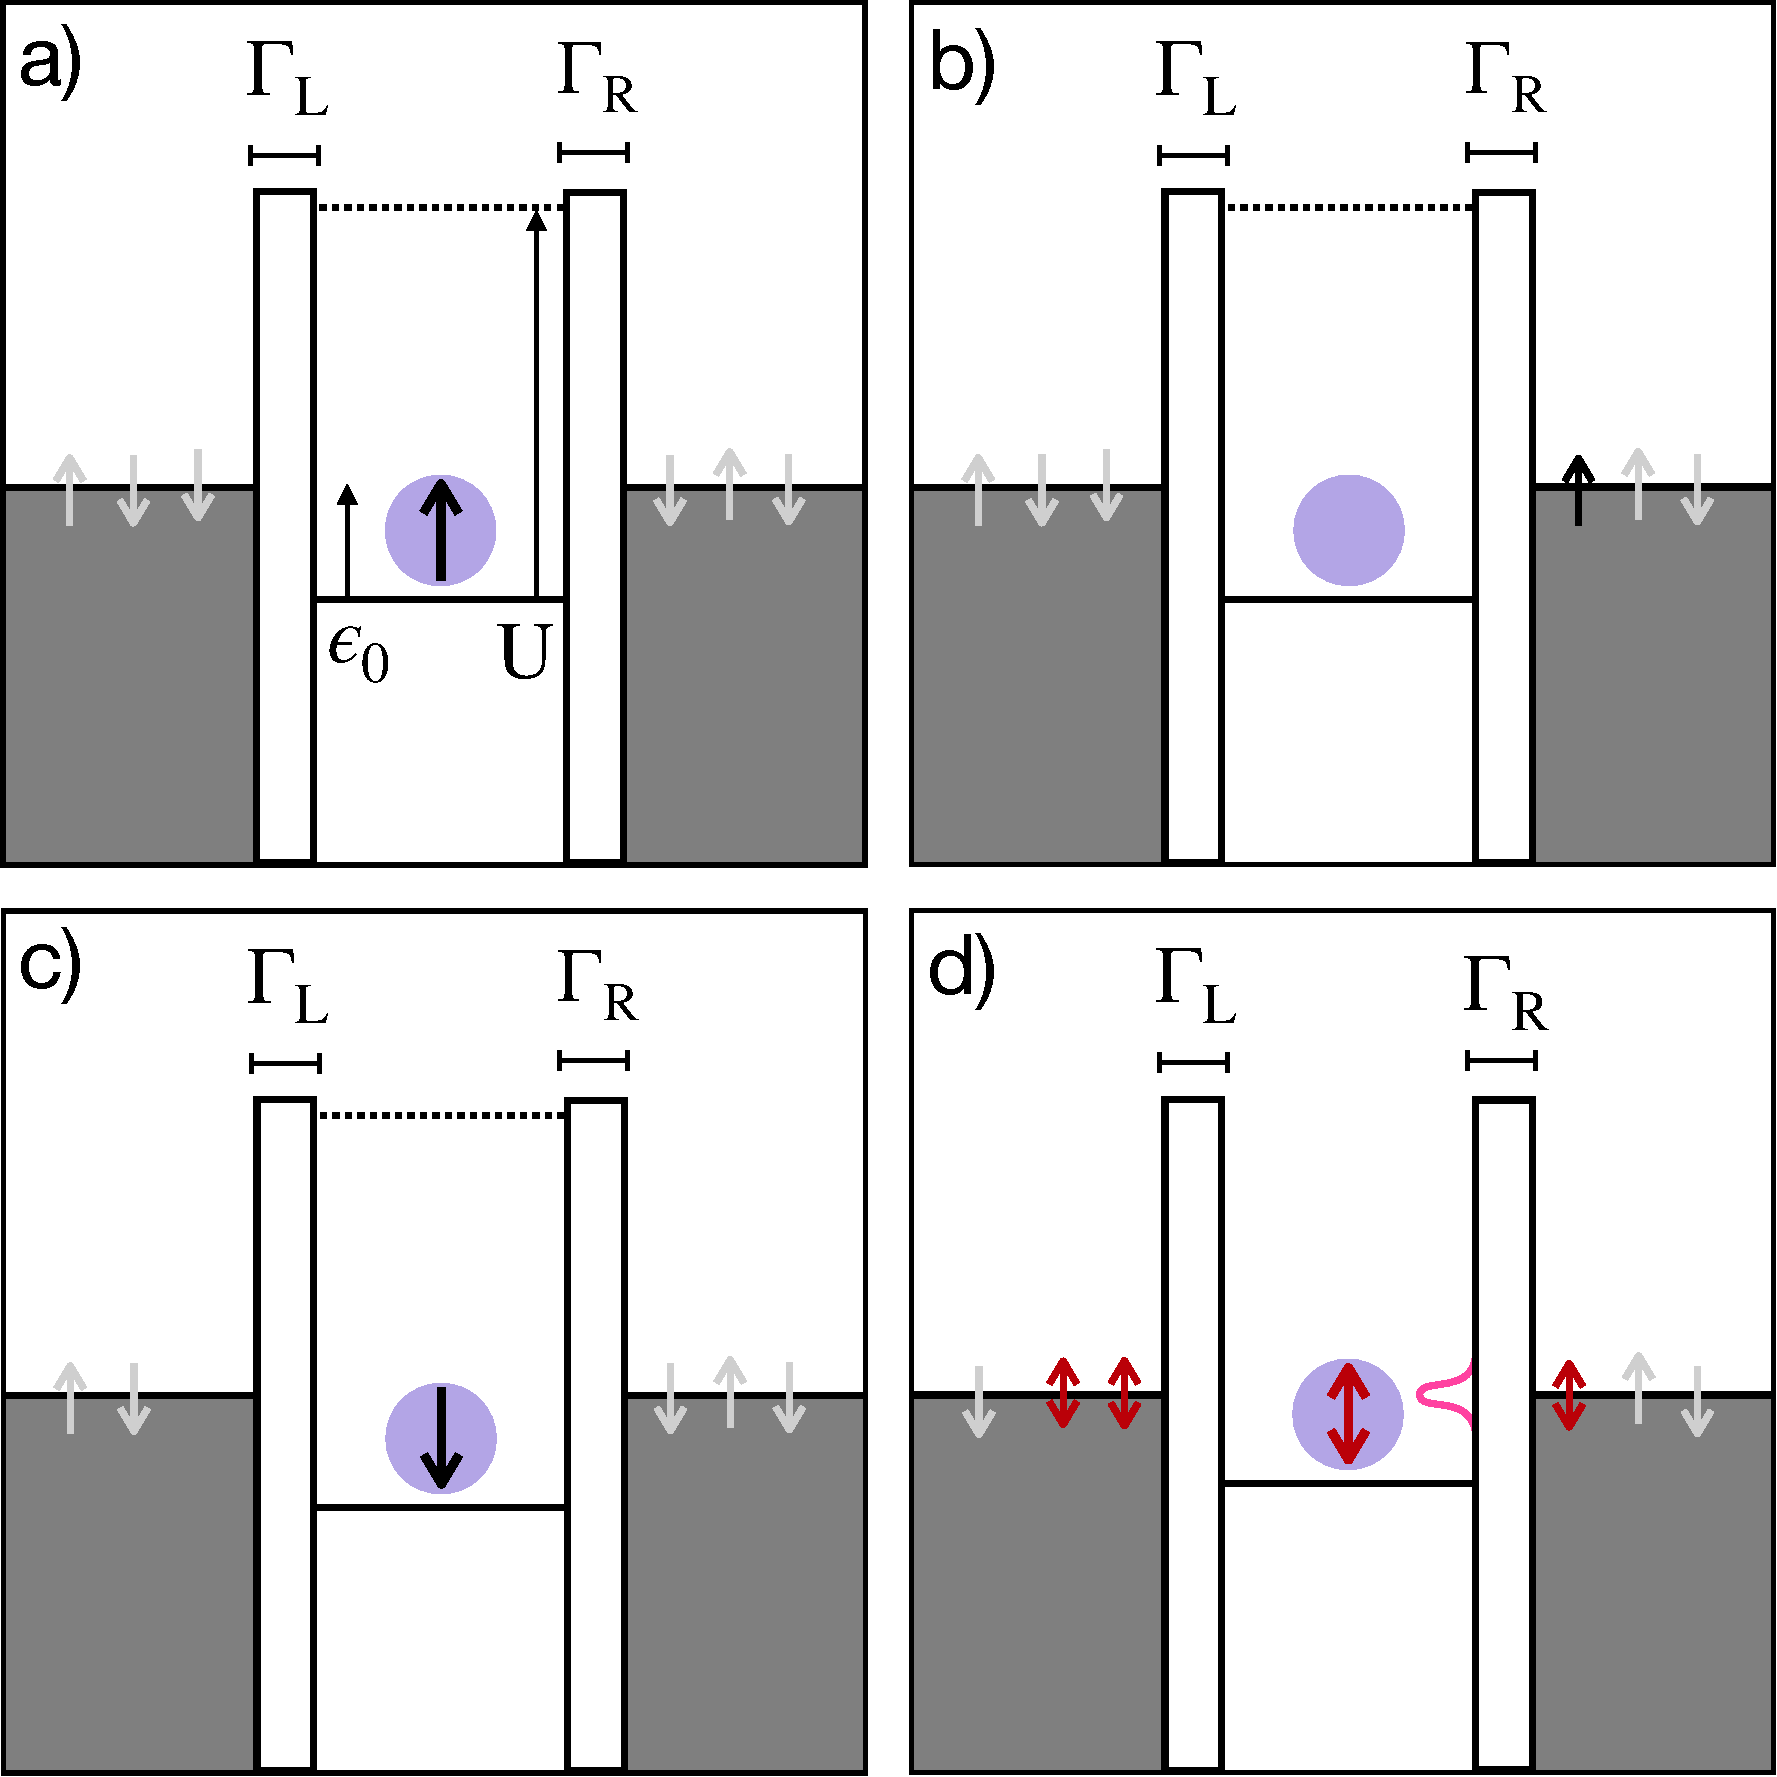
\includegraphics[width=0.75\textwidth]{figures/ch2/figure11.pdf}
  \caption[Kondo Effect Illustration : Quantum Dot]{\label{fig:ch2/kondo_dot_diagram} 
  % For some options that work with pdf\LaTeX, please see this discussion:
  %  \url{http://tex.stackexchange.com/questions/11839}. 
  A Coulomb blockade energy diagram illustrates the formation of a Kondo singlet in a quantum dot. Here, the dot acts as a localised spin. The dark grey represents the continuous energy level of electrons in the leads. The white rectangles represent tunnel barriers between the quantum dot and leads. The rate of tunnelling is denoted by the parameter $\Gamma$; the wider (narrower) the barrier, the smaller (larger) the rate of tunnelling. (\textbf{a}) The quantum dot has a one-spin degenerate energy level with dot energy $\mathrm{\epsilon_0}$, occupied by a single electron. The charging energy, $\mathrm{U}$, separates the next energy level. According to Fig.~\ref{fig:ch1/dot_intro}, zero conductance is expected through the quantum dot. However, (\textbf{b},\textbf{c}) depict a possible virtual tunnelling event. Here, the spin-up electron tunnels out of the dot, and a spin-down electron tunnels into the dot within a short time. (\textbf{d}) Many virtual tunnelling events involving possible spin flips lead to a correlated state, the Kondo singlet. This state is pictured as a narrow density of states formed at the Fermi energy of the leads. If a Kondo singlet has been formed, enhanced conductance is measured through the quantum dot, even as the dot energy $\epsilon_0$ is below the energy level of the leads. Note the formation of the Kondo singlet requires an odd number of electrons in the quantum dot.
   }
 \end{center}
\end{figure}


Until the late 1990s, theorists primarily explored the Kondo effect due to the difficulty of experimentally controlling the Kondo state~\cite{kondo_review}. However, after advances in quantum dot design, the potential for precise in situ control was irresistible, and the first measurement of a Kondo singlet was in 1998~\cite{goldhaber_first_kondo}. Around this time a scanning tunneling microscope (STM) was also used to study the Kondo effect~\cite{stm_kondo}.

In quantum dots, an odd number of electrons results in an unpaired electron that acts as the magnetic impurity in bulk metals. Like bulk metals, the conduction electrons in the 2DEG can interact with the net spin in the quantum dot. The advantage of studying the Kondo effect in quantum dots comes from the in situ control over the coupling strength, voltage bias, and energy level of the magnetic impurity.

The formation of a Kondo singlet in quantum dots is shown in Fig.~\ref{fig:ch2/kondo_dot_diagram}. 
Suppose the dot energy of the quantum dot is far below the Fermi energy of the leads. In that case, the electron is not expected to tunnel out of the dot as it does not have the required energy to reach the available empty energy levels in the leads (Fig.~\ref{fig:ch1/dot_intro}). However, a second-order tunnelling process can occur where the electron in the quantum dot tunnels into the leads. If the electron in the quantum dot tunnels into the leads (Fig.~\ref{fig:ch2/kondo_dot_diagram}\textbf{b}) another electron must tunnel into the quantum dot within a timescale limited by Heisenberg’s uncertainty principle (Fig.~\ref{fig:ch2/kondo_dot_diagram}\textbf{c}). This second-order process can result in a spin flip of the impurity. Many of these virtual tunnelling events will lead to the formation of a singlet state illustrated in Fig.~\ref{fig:ch2/kondo_dot_diagram}\textbf{d}), resulting in a narrow density of states formed at the Fermi energy of the leads. 


 \begin{figure}[!hbt]
 \begin{center}
%% includegraphics: comment the following if not using the graphicx package
  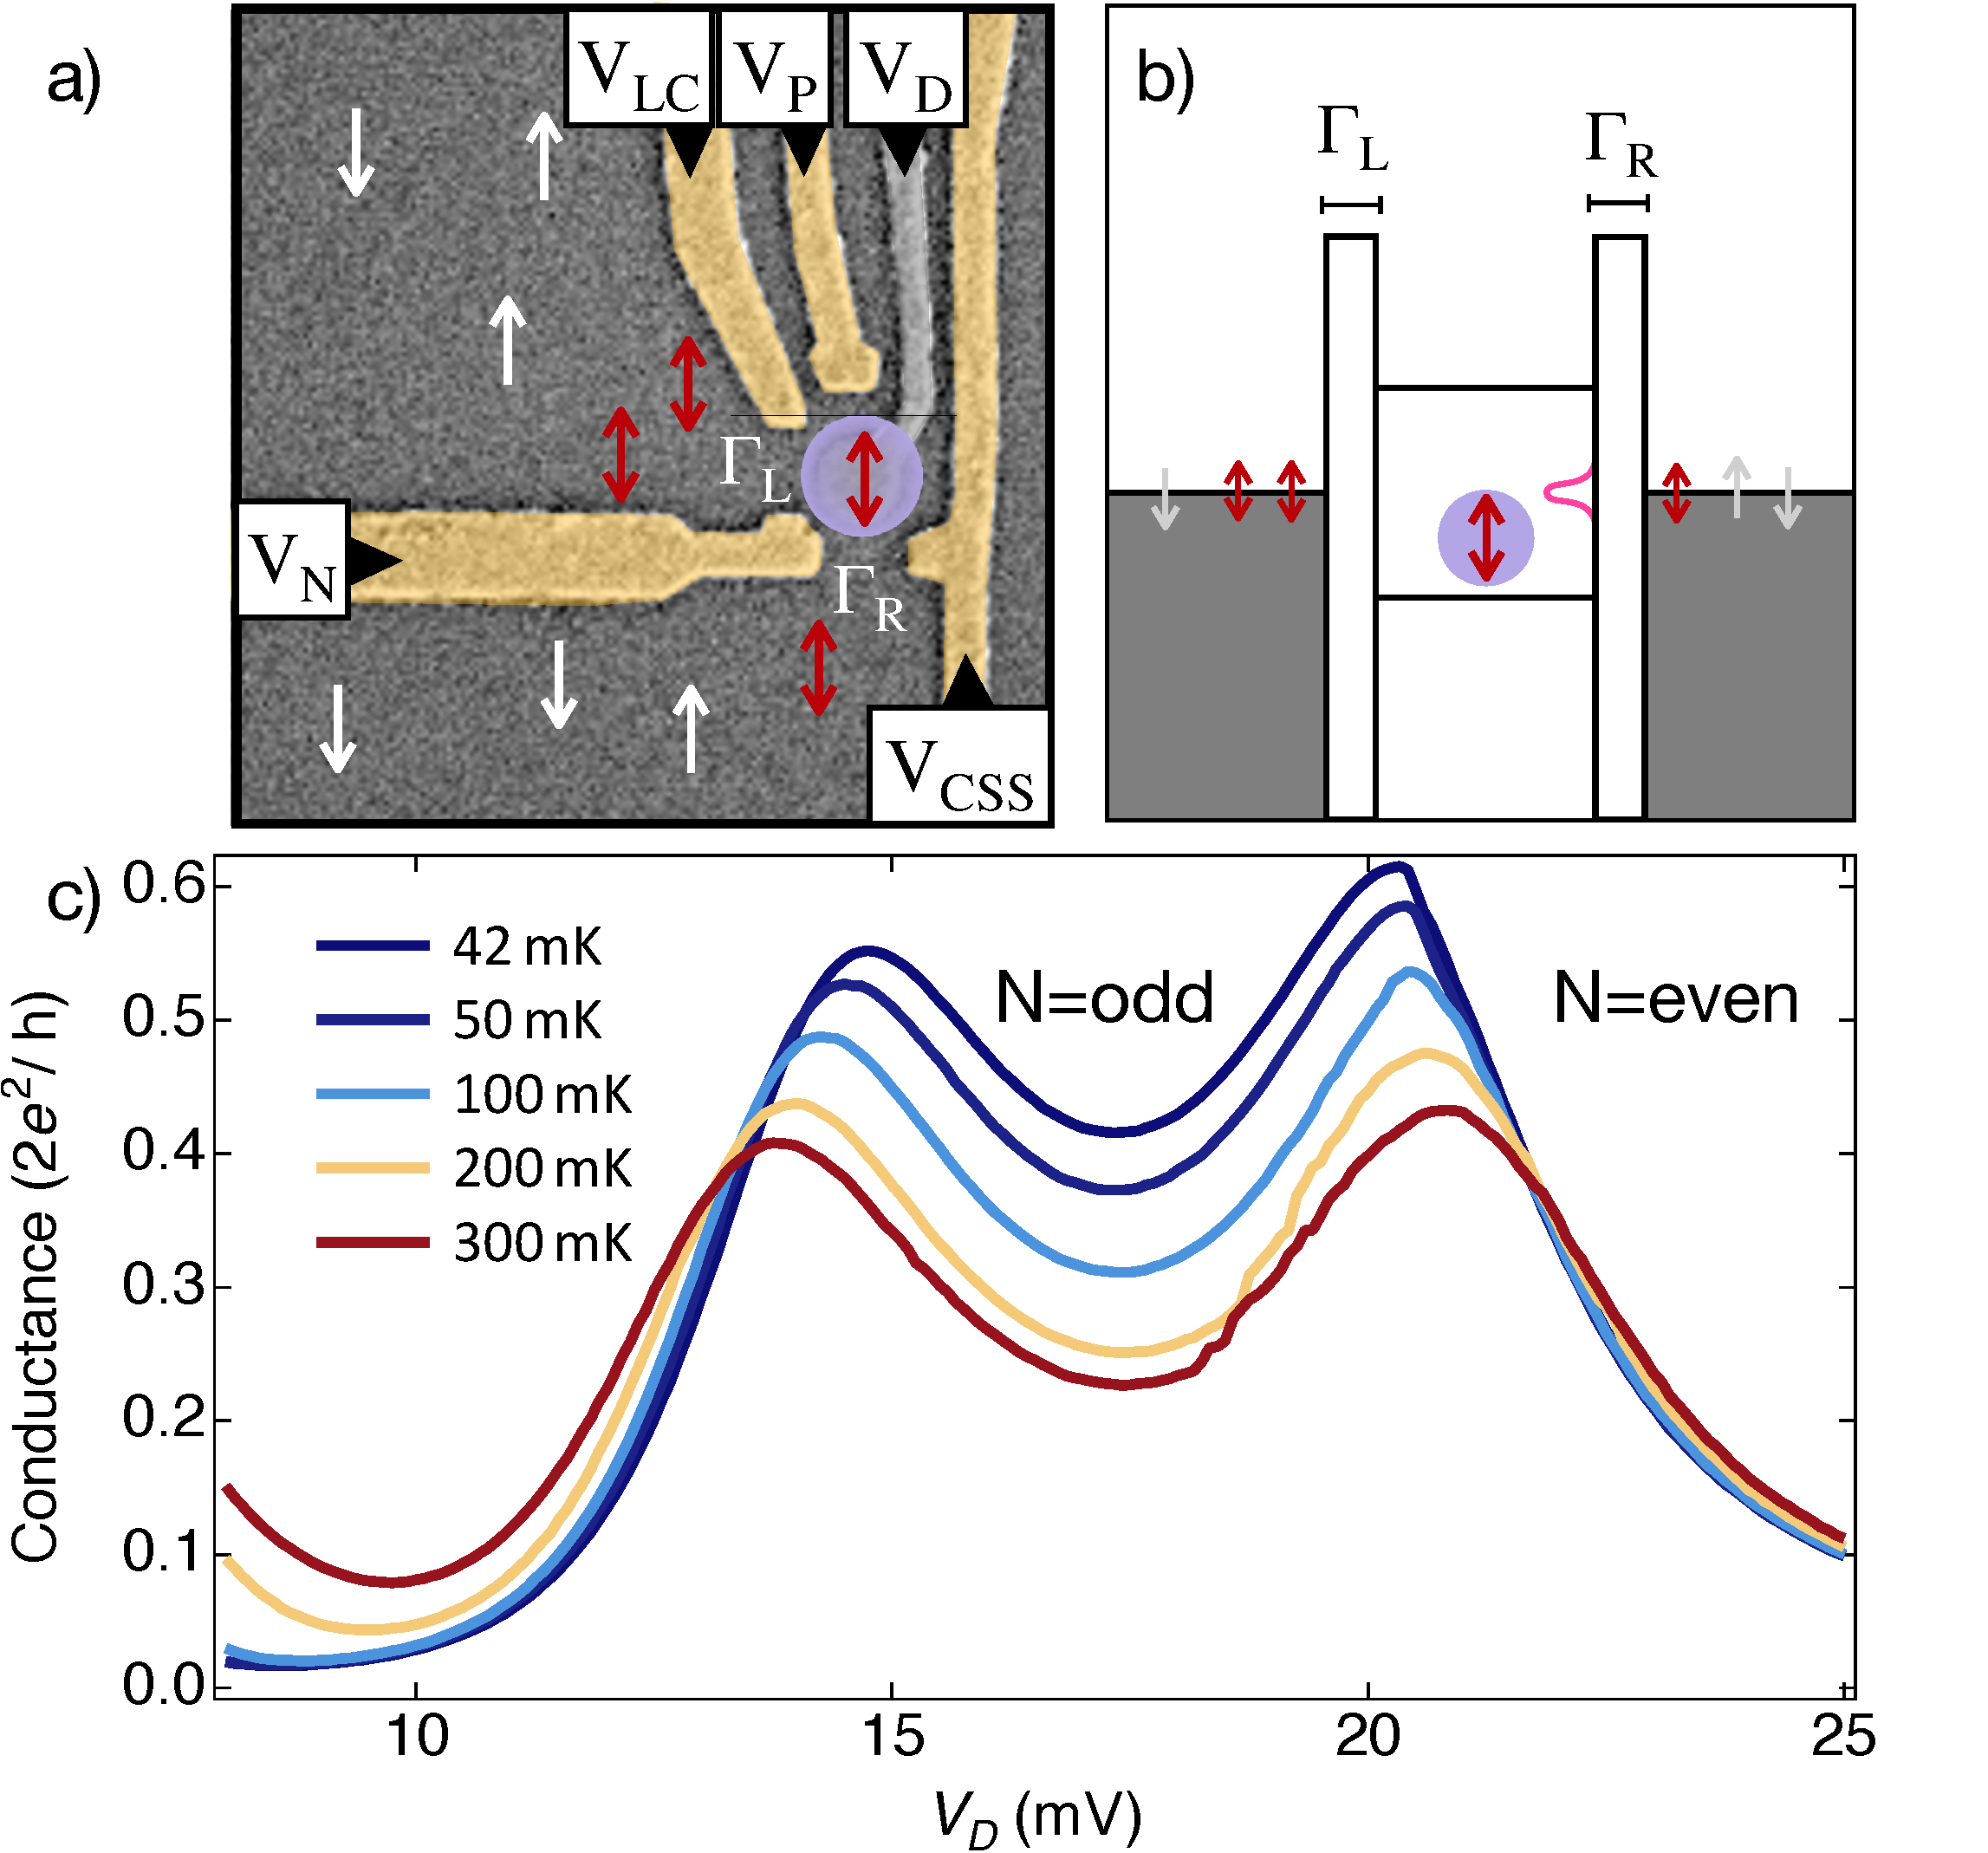
\includegraphics[width=0.9\textwidth]{figures/ch2/figure12.pdf}
  \caption[Kondo Effect in a Strongly Coupled Quantum Dot]{\label{fig:ch2/kondo_regime_conductance} 
  % For some options that work with pdf\LaTeX, please see this discussion:
  %  \url{http://tex.stackexchange.com/questions/11839}. 
  (\textbf{a}) SEM image of the gates used to define a quantum dot. The dot contains an odd number of electrons, and the tunnel barriers are tuned to form a Kondo singlet. \textbf{b}) Coulomb blockade energy diagram picture of a Kondo singlet. As the dot energy falls below the energy level of the leads, there is enhanced conductance due to virtual tunnelling events through the quantum dot. (\textbf{c}) Data showing the temperature dependence of conductance through a quantum dot when a Kondo singlet is formed. In the even occupied sides, conductance decreases as the temperature is lowered. With odd occupation, a Kondo singlet forms, and conductance increases with decreasing temperature.}
 \end{center}
\end{figure}



 Unlike the resistivity increase in bulk metals, the presence of a Kondo singlet leads to enhanced conductance through the quantum dot. Fig.~\ref{fig:ch2/kondo_regime_conductance}\textbf{c}) shows a measurement of conductance at a range of temperatures. At odd occupation, a Kondo singlet is formed and conductance through the quantum dot increases with decreasing temperature. This enhancement of conductance is dependent on a single parameter which sets the energy scale, the Kondo temperature $\mathrm{T_K}$. The Kondo temperature is given by Haldane~\cite{Haldane1978, kondo_thesis_stuttgart} as,
 

\begin{equation}\label{eq:kondo_temp}
 \mathrm{T_K} = 
 \frac{\sqrt{\hbar\Gamma \mathrm{U}}}{2\mathrm{k_B}}
 e^{\pi \epsilon_0 (\epsilon_0 + \mathrm{U})/\hbar\Gamma\mathrm{U}}
\end{equation}

 \noindent here $\epsilon_0$ is the dot energy, $\mathrm{U}$ the charging energy and $\Gamma$ is the coupling of the dot to both source and drain leads, $\mathrm{\Gamma = \Gamma_L + \Gamma_R}$. 
 An important realisation from Eq.~\ref{eq:kondo_temp} is that the Kondo temperature is not a constant value but is dependent on parameters that can be controlled in an experiment. 
 From Fig.~\ref{fig:ch2/kondo_regime_conductance}\textbf{a}) the dot energy is controlled by V\textsubscript{P} or V\textsubscript{D} and the coupling by V\textsubscript{LC}, V\textsubscript{N} or V\textsubscript{CSS}.
This expression for the Kondo temperature (Eq.~\ref{eq:kondo_temp}) only holds in the `Kondo regime'. The Kondo regime is characterised by $\tilde{\epsilon}_0<<-0.5$ where $\tilde{\epsilon}\equiv \epsilon_0/\Gamma$. Qualitatively, this regime is satisfied when the full charge of the electron is in the quantum dot. Consequently, as the dot energy is raised so that only a fraction of the electron charge is localised in the quantum dot, this expression for the Kondo temperature breaks down. However, the quantum dot still mainly exhibits a net spin, and Kondo enhancement remains. Importantly, the Kondo temperature increases as the dot energy approaches the Fermi energy of the leads~\cite{goldhaber_mv}, although it may not be exponential in form. This `turning on' of the Kondo effect close to the Fermi energy of the leads is the basis for measurements in the following Chapter~\ref{cha:mixed_valence_conductance}.
 

Many early measurements on the Kondo effect in quantum dots used very strong couplings, so the system temperature remained below the Kondo temperature deep into the Kondo regime~\cite{kondo_unitary}. Such studies examined temperature dependence of the conductance in the Coulomb blockade valley where the conductance dependence on temperature is non-monotonic and has a minimum at finite temperatures~\cite{Pustilnik2004}. The Kondo temperature (Eq.~\ref{eq:kondo_temp}) sets a new many-body scale in the Kondo regime. The Kondo temperature can be used to normalise the conductance such that it is independent of other energy scales $\Gamma$, $\mathrm{U}$, and $\tilde{\epsilon}_0$~\cite{costi_kondo_mv_eo_regime}. This normalisation is given as, 

\begin{equation}\label{eq:kondo_conductance}
 \mathrm{G(T)} =
 \mathrm{G_0}
 \left(
 \frac{\mathrm{T_K'^{2}}}{\mathrm{T^2} + \mathrm{T_K'^{2}}}
 \right)^\mathrm{s}
\end{equation}

\noindent here $\mathrm{T_K'^{2}} = \mathrm{T_K}/\sqrt{2^{\mathrm{1/s}}-1}$ and $\mathrm{s} \approx 0.20$ for a spin 1/2 system in the Kondo regime~\cite{goldhaber_mv}. The parameter $\mathrm{s}$ determines the steepness of the conductance drop with increasing temperature. The one-parameter scaling of the conductance in the Kondo regime is used as one of the demonstrations of the Kondo effect. Other measurements include a zero bias peak in the Coulomb blockade valley~\cite{kondo_unitary} and a splitting of this zero bias peak with magnetic field~\cite{cronenwett_tunable_kondo}. 

Other efforts have been made to explore the Kondo effect with less strong coupling. In this regime, the conductance in the middle of the Coulomb blockade valley does not increase with decreasing temperature~\cite{goldhaber_mv}. However, the dot energy of the quantum dot can be tuned to increase the Kondo temperature. As the dot energy approaches the Fermi energy of the leads, a conductance enhancement due to the Kondo effect can be recovered at sufficiently low system temperatures. The next Chapter~\ref{cha:mixed_valence_conductance} will focus on this regime of weaker coupling.


